% Options for packages loaded elsewhere
\PassOptionsToPackage{unicode=true}{hyperref}
\PassOptionsToPackage{hyphens}{url}
%
\documentclass[
]{article}
\usepackage{lmodern}
\usepackage{amssymb,amsmath}
\usepackage{ifxetex,ifluatex}
\ifnum 0\ifxetex 1\fi\ifluatex 1\fi=0 % if pdftex
  \usepackage[T1]{fontenc}
  \usepackage[utf8]{inputenc}
  \usepackage{textcomp} % provides euro and other symbols
\else % if luatex or xelatex
  \usepackage{unicode-math}
  \defaultfontfeatures{Scale=MatchLowercase}
  \defaultfontfeatures[\rmfamily]{Ligatures=TeX,Scale=1}
\fi
% Use upquote if available, for straight quotes in verbatim environments
\IfFileExists{upquote.sty}{\usepackage{upquote}}{}
\IfFileExists{microtype.sty}{% use microtype if available
  \usepackage[]{microtype}
  \UseMicrotypeSet[protrusion]{basicmath} % disable protrusion for tt fonts
}{}
\makeatletter
\@ifundefined{KOMAClassName}{% if non-KOMA class
  \IfFileExists{parskip.sty}{%
    \usepackage{parskip}
  }{% else
    \setlength{\parindent}{0pt}
    \setlength{\parskip}{6pt plus 2pt minus 1pt}}
}{% if KOMA class
  \KOMAoptions{parskip=half}}
\makeatother
\usepackage{xcolor}
\IfFileExists{xurl.sty}{\usepackage{xurl}}{} % add URL line breaks if available
\IfFileExists{bookmark.sty}{\usepackage{bookmark}}{\usepackage{hyperref}}
\hypersetup{
  pdftitle={STAT\_205\_HW2},
  pdfauthor={HONGLEI REN},
  hidelinks,
}
\urlstyle{same} % disable monospaced font for URLs
\usepackage[margin=1in]{geometry}
\usepackage{color}
\usepackage{fancyvrb}
\newcommand{\VerbBar}{|}
\newcommand{\VERB}{\Verb[commandchars=\\\{\}]}
\DefineVerbatimEnvironment{Highlighting}{Verbatim}{commandchars=\\\{\}}
% Add ',fontsize=\small' for more characters per line
\usepackage{framed}
\definecolor{shadecolor}{RGB}{248,248,248}
\newenvironment{Shaded}{\begin{snugshade}}{\end{snugshade}}
\newcommand{\AlertTok}[1]{\textcolor[rgb]{0.94,0.16,0.16}{#1}}
\newcommand{\AnnotationTok}[1]{\textcolor[rgb]{0.56,0.35,0.01}{\textbf{\textit{#1}}}}
\newcommand{\AttributeTok}[1]{\textcolor[rgb]{0.77,0.63,0.00}{#1}}
\newcommand{\BaseNTok}[1]{\textcolor[rgb]{0.00,0.00,0.81}{#1}}
\newcommand{\BuiltInTok}[1]{#1}
\newcommand{\CharTok}[1]{\textcolor[rgb]{0.31,0.60,0.02}{#1}}
\newcommand{\CommentTok}[1]{\textcolor[rgb]{0.56,0.35,0.01}{\textit{#1}}}
\newcommand{\CommentVarTok}[1]{\textcolor[rgb]{0.56,0.35,0.01}{\textbf{\textit{#1}}}}
\newcommand{\ConstantTok}[1]{\textcolor[rgb]{0.00,0.00,0.00}{#1}}
\newcommand{\ControlFlowTok}[1]{\textcolor[rgb]{0.13,0.29,0.53}{\textbf{#1}}}
\newcommand{\DataTypeTok}[1]{\textcolor[rgb]{0.13,0.29,0.53}{#1}}
\newcommand{\DecValTok}[1]{\textcolor[rgb]{0.00,0.00,0.81}{#1}}
\newcommand{\DocumentationTok}[1]{\textcolor[rgb]{0.56,0.35,0.01}{\textbf{\textit{#1}}}}
\newcommand{\ErrorTok}[1]{\textcolor[rgb]{0.64,0.00,0.00}{\textbf{#1}}}
\newcommand{\ExtensionTok}[1]{#1}
\newcommand{\FloatTok}[1]{\textcolor[rgb]{0.00,0.00,0.81}{#1}}
\newcommand{\FunctionTok}[1]{\textcolor[rgb]{0.00,0.00,0.00}{#1}}
\newcommand{\ImportTok}[1]{#1}
\newcommand{\InformationTok}[1]{\textcolor[rgb]{0.56,0.35,0.01}{\textbf{\textit{#1}}}}
\newcommand{\KeywordTok}[1]{\textcolor[rgb]{0.13,0.29,0.53}{\textbf{#1}}}
\newcommand{\NormalTok}[1]{#1}
\newcommand{\OperatorTok}[1]{\textcolor[rgb]{0.81,0.36,0.00}{\textbf{#1}}}
\newcommand{\OtherTok}[1]{\textcolor[rgb]{0.56,0.35,0.01}{#1}}
\newcommand{\PreprocessorTok}[1]{\textcolor[rgb]{0.56,0.35,0.01}{\textit{#1}}}
\newcommand{\RegionMarkerTok}[1]{#1}
\newcommand{\SpecialCharTok}[1]{\textcolor[rgb]{0.00,0.00,0.00}{#1}}
\newcommand{\SpecialStringTok}[1]{\textcolor[rgb]{0.31,0.60,0.02}{#1}}
\newcommand{\StringTok}[1]{\textcolor[rgb]{0.31,0.60,0.02}{#1}}
\newcommand{\VariableTok}[1]{\textcolor[rgb]{0.00,0.00,0.00}{#1}}
\newcommand{\VerbatimStringTok}[1]{\textcolor[rgb]{0.31,0.60,0.02}{#1}}
\newcommand{\WarningTok}[1]{\textcolor[rgb]{0.56,0.35,0.01}{\textbf{\textit{#1}}}}
\usepackage{graphicx,grffile}
\makeatletter
\def\maxwidth{\ifdim\Gin@nat@width>\linewidth\linewidth\else\Gin@nat@width\fi}
\def\maxheight{\ifdim\Gin@nat@height>\textheight\textheight\else\Gin@nat@height\fi}
\makeatother
% Scale images if necessary, so that they will not overflow the page
% margins by default, and it is still possible to overwrite the defaults
% using explicit options in \includegraphics[width, height, ...]{}
\setkeys{Gin}{width=\maxwidth,height=\maxheight,keepaspectratio}
\setlength{\emergencystretch}{3em} % prevent overfull lines
\providecommand{\tightlist}{%
  \setlength{\itemsep}{0pt}\setlength{\parskip}{0pt}}
\setcounter{secnumdepth}{-\maxdimen} % remove section numbering
% Redefines (sub)paragraphs to behave more like sections
\ifx\paragraph\undefined\else
  \let\oldparagraph\paragraph
  \renewcommand{\paragraph}[1]{\oldparagraph{#1}\mbox{}}
\fi
\ifx\subparagraph\undefined\else
  \let\oldsubparagraph\subparagraph
  \renewcommand{\subparagraph}[1]{\oldsubparagraph{#1}\mbox{}}
\fi

% Set default figure placement to htbp
\makeatletter
\def\fps@figure{htbp}
\makeatother


\title{STAT\_205\_HW2}
\author{HONGLEI REN}
\date{1/20/2020}

\begin{document}
\maketitle

\hypertarget{problem-1}{%
\subsection{Problem 1}\label{problem-1}}

\hypertarget{propose-a-conjugate-normal-prior-mu-sim-nmu_0-tau_0}{%
\subsubsection{\texorpdfstring{1.1 Propose a conjugate Normal Prior
\(\mu \sim N(\mu_0, \tau_0)\)}{1.1 Propose a conjugate Normal Prior \textbackslash mu \textbackslash sim N(\textbackslash mu\_0, \textbackslash tau\_0)}}\label{propose-a-conjugate-normal-prior-mu-sim-nmu_0-tau_0}}

According to the percentile table of standard normal distribution, we
know that:

\[z = \frac{x - \mu_0}{\sqrt{\tau_0}} = \frac{42 - 40}{\sqrt{\tau_0}} = \frac{2}{\sqrt{\tau_0}}= 1.96\],
and we got \(\tau_0 = (\frac{2}{1.96})^2\). Therefore, the Normal prior
is \(\mu \sim N(40, (\frac{2}{1.96})^2)\).

\hypertarget{the-posterior-expectation}{%
\subsubsection{1.2 The Posterior
Expectation}\label{the-posterior-expectation}}

Suppose
\(\tau_0 = \frac{\sigma^2}{m} = \frac{10^2}{m} = (\frac{2}{1.96})^2\),
therefore, \(m = 96.04\).

Then, we have
\(Y|\mu, \sigma^2 \sim Normal(\mu, 10^2), \mu \sim N(40, \frac{10^2}{96.04})\).
The posterior
is:\[\mu|Y \sim N(w\overline{Y} + (1 - w) \mu_0, \frac{\sigma^2}{n + m})\],
where \(w = \frac{n}{n + m}\), \(\overline{Y} = 45.283\) is the sample
mean.

Therefore, the posterior mean is \(40.586\), which is very close to the
prior mean although the sample mean \(45.283\) is much higher, and this
is caused by a strong prior.

In our case, the relative contribution of prior is \(0.89\) and data for
posterior expectation is \(0.11\).

\hypertarget{the-posterior-distribution}{%
\subsubsection{1.3 The Posterior
Distribution}\label{the-posterior-distribution}}

From the figure below, we can see that posterior distribution \(mu\)
shifts towards right of the prior, which means the data suggest average
snowfall observed are higher than our prior knowledge.

\begin{Shaded}
\begin{Highlighting}[]
\CommentTok{#Data}
\NormalTok{snowfall =}\StringTok{ }\KeywordTok{c}\NormalTok{(}\FloatTok{38.6}\NormalTok{, }\FloatTok{42.4}\NormalTok{, }\FloatTok{57.5}\NormalTok{, }\FloatTok{40.5}\NormalTok{, }\FloatTok{51.7}\NormalTok{, }\FloatTok{67.1}\NormalTok{, }\FloatTok{33.4}\NormalTok{, }\FloatTok{60.9}\NormalTok{, }\FloatTok{64.1}\NormalTok{, }\FloatTok{40.1}\NormalTok{, }\FloatTok{40.7}\NormalTok{, }\FloatTok{6.4}\NormalTok{)}
\NormalTok{mean_snowfall =}\StringTok{ }\KeywordTok{mean}\NormalTok{(snowfall)}

\CommentTok{#Params}
\NormalTok{n =}\StringTok{ }\KeywordTok{length}\NormalTok{(snowfall)}
\NormalTok{m =}\StringTok{ }\FloatTok{96.04}
\NormalTok{mu0 =}\StringTok{ }\DecValTok{40}
\NormalTok{sigma =}\StringTok{ }\DecValTok{10}
\NormalTok{w =}\StringTok{ }\NormalTok{n }\OperatorTok{/}\StringTok{ }\NormalTok{(n }\OperatorTok{+}\StringTok{ }\NormalTok{m)}
\NormalTok{mu =}\StringTok{ }\KeywordTok{seq}\NormalTok{(}\DecValTok{35}\NormalTok{, }\DecValTok{45}\NormalTok{, }\FloatTok{0.5}\NormalTok{)}

\CommentTok{# Calculate prior and posterior}
\NormalTok{prior_mu =}\StringTok{ }\KeywordTok{dnorm}\NormalTok{(mu, }\DataTypeTok{mean =}\NormalTok{ mu0, }\DataTypeTok{sd=}\NormalTok{ (sigma}\OperatorTok{^}\DecValTok{2}\NormalTok{) }\OperatorTok{/}\StringTok{ }\NormalTok{m)}
\NormalTok{posterior_mean =}\StringTok{ }\NormalTok{w }\OperatorTok{*}\StringTok{ }\NormalTok{mean_snowfall }\OperatorTok{+}\StringTok{ }\NormalTok{(}\DecValTok{1} \OperatorTok{-}\StringTok{ }\NormalTok{w) }\OperatorTok{*}\StringTok{ }\NormalTok{mu0}
\NormalTok{posterior_sd =}\StringTok{ }\NormalTok{(sigma}\OperatorTok{^}\DecValTok{2}\NormalTok{) }\OperatorTok{/}\StringTok{ }\NormalTok{(n }\OperatorTok{+}\StringTok{ }\NormalTok{m)}
\NormalTok{posterior_mu =}\StringTok{ }\KeywordTok{dnorm}\NormalTok{(mu, }\DataTypeTok{mean =}\NormalTok{ posterior_mean, }\DataTypeTok{sd=}\NormalTok{ posterior_sd)}

\CommentTok{# Plotting}
\KeywordTok{plot}\NormalTok{(mu, prior_mu}\OperatorTok{/}\KeywordTok{sum}\NormalTok{(prior_mu),}\DataTypeTok{col=}\StringTok{"blue"}\NormalTok{, }\DataTypeTok{type=}\StringTok{"b"}\NormalTok{, }\DataTypeTok{xlab =} \KeywordTok{expression}\NormalTok{(mu), }\DataTypeTok{ylab =} \StringTok{"probability"}\NormalTok{, }\DataTypeTok{ylim=}\KeywordTok{range}\NormalTok{(}\KeywordTok{c}\NormalTok{(}\DecValTok{0}\NormalTok{,}\FloatTok{0.3}\NormalTok{)))}
\KeywordTok{par}\NormalTok{(}\DataTypeTok{new=}\OtherTok{TRUE}\NormalTok{)}
\KeywordTok{plot}\NormalTok{(mu, posterior_mu}\OperatorTok{/}\KeywordTok{sum}\NormalTok{(posterior_mu), }\DataTypeTok{col=}\StringTok{"red"}\NormalTok{, }\DataTypeTok{type=}\StringTok{"b"}\NormalTok{, }\DataTypeTok{xlab =} \KeywordTok{expression}\NormalTok{(mu), }\DataTypeTok{ylab =} \StringTok{"probability"}\NormalTok{, }\DataTypeTok{ylim=}\KeywordTok{range}\NormalTok{(}\KeywordTok{c}\NormalTok{(}\DecValTok{0}\NormalTok{,}\FloatTok{0.3}\NormalTok{)))}
\KeywordTok{legend}\NormalTok{(}\DecValTok{35}\NormalTok{, }\FloatTok{0.28}\NormalTok{, }\DataTypeTok{legend=}\KeywordTok{c}\NormalTok{(}\StringTok{"prior"}\NormalTok{, }\StringTok{"posterior"}\NormalTok{),}
       \DataTypeTok{col=}\KeywordTok{c}\NormalTok{(}\StringTok{"blue"}\NormalTok{, }\StringTok{"red"}\NormalTok{), }\DataTypeTok{lty=}\DecValTok{1}\OperatorTok{:}\DecValTok{1}\NormalTok{, }\DataTypeTok{cex=}\FloatTok{0.8}\NormalTok{)}
\end{Highlighting}
\end{Shaded}

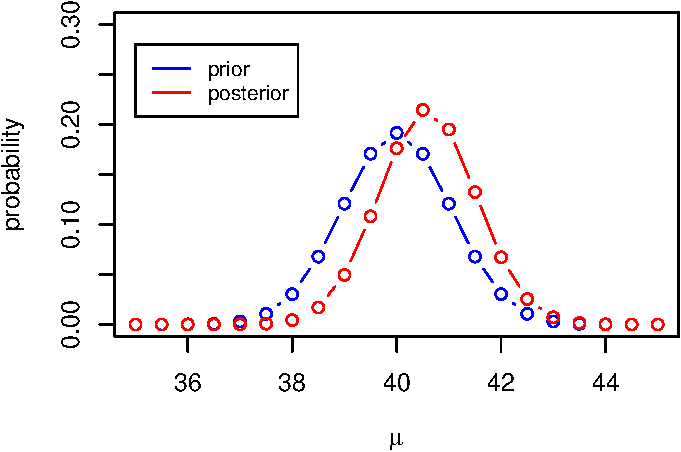
\includegraphics{STAT_205_HW2_files/figure-latex/unnamed-chunk-2-1.pdf}

\hypertarget{quantiles-of-posterior-distribution}{%
\subsubsection{1.4 Quantiles of Posterior
Distribution}\label{quantiles-of-posterior-distribution}}

\begin{Shaded}
\begin{Highlighting}[]
\NormalTok{S =}\StringTok{ }\DecValTok{100000} \CommentTok{#Sample size}
\NormalTok{mu_star =}\StringTok{ }\KeywordTok{rnorm}\NormalTok{(S, posterior_mean, posterior_sd)}
\NormalTok{pct_}\DecValTok{10}\NormalTok{ =}\StringTok{ }\KeywordTok{quantile}\NormalTok{(mu_star, }\FloatTok{0.1}\NormalTok{)}
\NormalTok{pct_}\DecValTok{10}
\end{Highlighting}
\end{Shaded}

\begin{verbatim}
##      10% 
## 39.39856
\end{verbatim}

\begin{Shaded}
\begin{Highlighting}[]
\NormalTok{pct_}\DecValTok{90}\NormalTok{ =}\StringTok{ }\KeywordTok{quantile}\NormalTok{(mu_star, }\FloatTok{0.9}\NormalTok{)}
\NormalTok{pct_}\DecValTok{90}
\end{Highlighting}
\end{Shaded}

\begin{verbatim}
##      90% 
## 41.77723
\end{verbatim}

The \(10\%\) quantiles of the posterior distribution is 39.3985587 and
the and \(90\%\) percentile is 41.7772265.

\hypertarget{posterior-mean-of-logmu}{%
\subsubsection{\texorpdfstring{1.5 Posterior mean of
log(\(\mu\))}{1.5 Posterior mean of log(\textbackslash mu)}}\label{posterior-mean-of-logmu}}

\begin{Shaded}
\begin{Highlighting}[]
\NormalTok{S =}\StringTok{ }\DecValTok{100000} \CommentTok{#Sample size}
\NormalTok{mu_star =}\StringTok{ }\KeywordTok{rnorm}\NormalTok{(S, posterior_mean, posterior_sd)}
\NormalTok{log_mu =}\StringTok{ }\KeywordTok{log}\NormalTok{(mu_star)}
\NormalTok{mean_log_mu =}\StringTok{ }\KeywordTok{mean}\NormalTok{(log_mu)}
\CommentTok{# Plotting}
\KeywordTok{plot}\NormalTok{(}\KeywordTok{density}\NormalTok{(log_mu),}\DataTypeTok{col=}\StringTok{"blue"}\NormalTok{, }\DataTypeTok{type=}\StringTok{"l"}\NormalTok{, }\DataTypeTok{xlab =} \KeywordTok{expression}\NormalTok{(}\KeywordTok{log}\NormalTok{(mu)), }\DataTypeTok{ylab =} \StringTok{"probability"}\NormalTok{, }\DataTypeTok{ylim=}\KeywordTok{range}\NormalTok{(}\KeywordTok{c}\NormalTok{(}\DecValTok{0}\NormalTok{, }\FloatTok{20.0}\NormalTok{)), }\DataTypeTok{main=}\KeywordTok{expression}\NormalTok{(}\StringTok{"PDF of "} \OperatorTok{~}\StringTok{ }\KeywordTok{log}\NormalTok{(mu)))}
\KeywordTok{legend}\NormalTok{(}\FloatTok{3.5}\NormalTok{, }\FloatTok{0.28}\NormalTok{, }\DataTypeTok{legend=}\KeywordTok{c}\NormalTok{(}\StringTok{"log(mu)"}\NormalTok{),}
       \DataTypeTok{col=}\KeywordTok{c}\NormalTok{(}\StringTok{"blue"}\NormalTok{), }\DataTypeTok{lty=}\DecValTok{1}\OperatorTok{:}\DecValTok{1}\NormalTok{, }\DataTypeTok{cex=}\FloatTok{0.8}\NormalTok{)}
\end{Highlighting}
\end{Shaded}

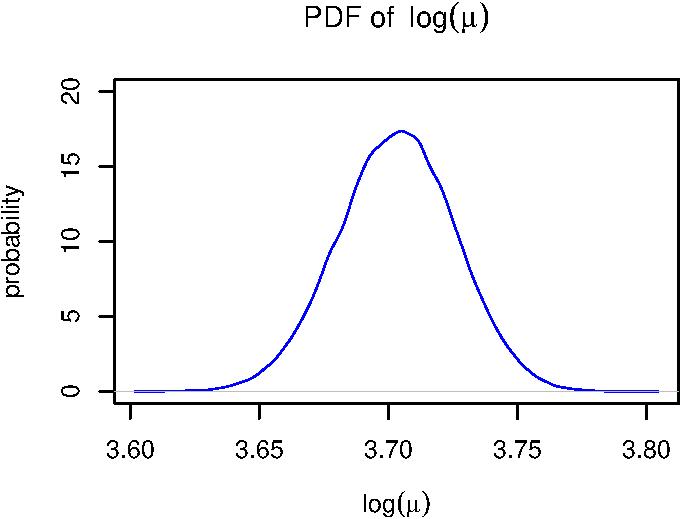
\includegraphics{STAT_205_HW2_files/figure-latex/unnamed-chunk-4-1.pdf}

\begin{Shaded}
\begin{Highlighting}[]
\NormalTok{mean_log_mu}
\end{Highlighting}
\end{Shaded}

\begin{verbatim}
## [1] 3.7032
\end{verbatim}

I first draw 10000 samples from the posterior distribution of \(\mu\),
and then perform a \textbf{log} transformation. Finally, I calculate the
mean from the log transformed samples of \(\mu\), and the posterior mean
of \(log(\mu)\) =3.7032001.

\hypertarget{problem-2}{%
\subsection{Problem 2}\label{problem-2}}

\hypertarget{derive-posterior}{%
\subsubsection{2.1 Derive posterior}\label{derive-posterior}}

The number of ASE for \(N\) patient follows
\(Y \sim Poisson(N \lambda)\) and \(\lambda \sim Gamma(a, b)\).

The likelihood function is :
\[f(Y|\lambda) \propto exp(-N \lambda) \lambda^Y\], where
\(N = 50, Y = 12 + 6*2 + 2 * 10 = 44\).

The prior function is:
\[\pi(\lambda) \propto exp(-b \lambda) \lambda^a\]

Therefore, the posterior is:
\[p(\lambda | Y) \propto exp(-\lambda) \lambda^Y exp(-b \lambda) \lambda^a \propto exp(-B \lambda) * \lambda^A\],
where \(A = a + Y\), \(B = b + N\). \[p(\lambda | Y) = Gamma(A, B)\].

\begin{Shaded}
\begin{Highlighting}[]
\NormalTok{N =}\StringTok{ }\DecValTok{9}
\NormalTok{Y =}\StringTok{ }\FloatTok{0.5}
\NormalTok{a =}\StringTok{ }\NormalTok{b =}\StringTok{ }\FloatTok{0.01}
\NormalTok{A =}\StringTok{ }\NormalTok{Y }\OperatorTok{+}\StringTok{ }\NormalTok{a}
\NormalTok{B =}\StringTok{ }\NormalTok{N }\OperatorTok{+}\StringTok{ }\NormalTok{b}
\NormalTok{lambdav =}\StringTok{ }\KeywordTok{seq}\NormalTok{(}\DecValTok{0}\NormalTok{, }\DecValTok{20}\NormalTok{, }\FloatTok{0.5}\NormalTok{)}
\NormalTok{prior_lambda =}\StringTok{ }\KeywordTok{dgamma}\NormalTok{(lambdav, }\DataTypeTok{shape =}\NormalTok{ a, }\DataTypeTok{scale=}\NormalTok{ b)}
\NormalTok{posterior_lambda =}\StringTok{ }\KeywordTok{dgamma}\NormalTok{(lambdav, }\DataTypeTok{shape =}\NormalTok{ A, }\DataTypeTok{scale=}\NormalTok{B)}

\CommentTok{# Plotting}
\KeywordTok{plot}\NormalTok{(lambdav, prior_lambda}\OperatorTok{/}\KeywordTok{sum}\NormalTok{(prior_lambda),}\DataTypeTok{col=}\StringTok{"blue"}\NormalTok{, }\DataTypeTok{type=}\StringTok{"b"}\NormalTok{, }\DataTypeTok{xlab =} \KeywordTok{expression}\NormalTok{(lambda), }\DataTypeTok{ylab =} \StringTok{"probability"}\NormalTok{, }\DataTypeTok{ylim=}\KeywordTok{range}\NormalTok{(}\KeywordTok{c}\NormalTok{(}\DecValTok{0}\NormalTok{,}\FloatTok{0.5}\NormalTok{)))}
\KeywordTok{par}\NormalTok{(}\DataTypeTok{new=}\OtherTok{TRUE}\NormalTok{)}
\KeywordTok{plot}\NormalTok{(lambdav, posterior_lambda}\OperatorTok{/}\KeywordTok{sum}\NormalTok{(posterior_lambda), }\DataTypeTok{col=}\StringTok{"red"}\NormalTok{, }\DataTypeTok{type=}\StringTok{"b"}\NormalTok{, }\DataTypeTok{xlab =} \KeywordTok{expression}\NormalTok{(lambda), }\DataTypeTok{ylab =} \StringTok{"probability"}\NormalTok{, }\DataTypeTok{ylim=}\KeywordTok{range}\NormalTok{(}\KeywordTok{c}\NormalTok{(}\DecValTok{0}\NormalTok{,}\FloatTok{0.5}\NormalTok{)))}
\KeywordTok{legend}\NormalTok{(}\DecValTok{0}\NormalTok{, }\FloatTok{0.28}\NormalTok{, }\DataTypeTok{legend=}\KeywordTok{c}\NormalTok{(}\StringTok{"prior"}\NormalTok{, }\StringTok{"posterior"}\NormalTok{),}
       \DataTypeTok{col=}\KeywordTok{c}\NormalTok{(}\StringTok{"blue"}\NormalTok{, }\StringTok{"red"}\NormalTok{), }\DataTypeTok{lty=}\DecValTok{1}\OperatorTok{:}\DecValTok{1}\NormalTok{, }\DataTypeTok{cex=}\FloatTok{0.8}\NormalTok{)}
\end{Highlighting}
\end{Shaded}

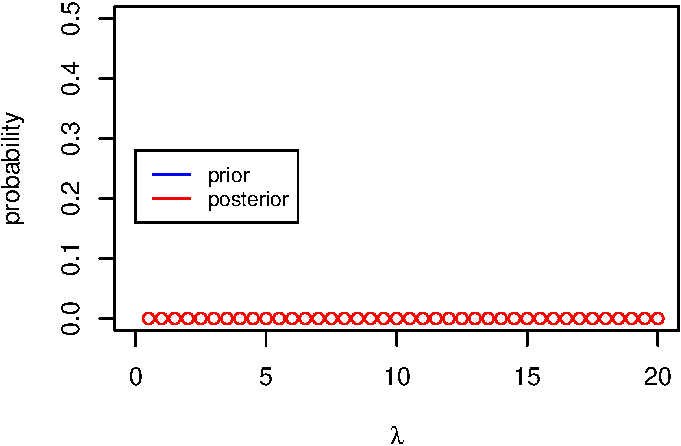
\includegraphics{STAT_205_HW2_files/figure-latex/unnamed-chunk-5-1.pdf}

\end{document}
